\documentclass[12pt, a4paper]{article}
\providecommand{\keywords}[1]{\textbf{Keywords:} #1}
%================================================================%
% PREAMBLE (PENGATURAN DASAR DOKUMEN)
%================================================================%
\usepackage[utf8]{inputenc}
\usepackage[T1]{fontenc}
\usepackage[indonesian]{babel}
\usepackage{newtxtext, newtxmath} % Font yang mirip Times New Roman
\usepackage[left=2.5cm, right=2.5cm, top=2.5cm, bottom=2.5cm]{geometry}
\usepackage{amsmath}
\usepackage{graphicx}
\usepackage{booktabs} % Untuk garis tabel yang lebih profesional
\usepackage{fancyhdr}
\usepackage[compact]{titlesec}
\usepackage{subcaption}
\usepackage[backend=biber, style=numeric, sorting=none]{biblatex}

% Ganti "referensi.bib" dengan nama file .bib Anda
\addbibresource{referensi.bib}

%================================================================%
% KUSTOMISASI LAYOUT & METADATA
%================================================================%

% Format judul seksi
\titleformat{\section}{\normalfont\large\bfseries}{\thesection.}{1em}{}
\titleformat{\subsection}{\normalfont\bfseries}{\thesubsection}{1em}{}

% Pengaturan Header dan Footer menggunakan fancyhdr
\pagestyle{fancy}
\fancyhf{} % Membersihkan semua field header/footer
\fancyhead[C]{\nouppercase{\leftmark}} % Judul seksi di tengah header
\fancyfoot[C]{\thepage} % Nomor halaman di tengah footer
\renewcommand{\headrulewidth}{0.4pt} % Garis tipis di bawah header
\renewcommand{\footrulewidth}{0pt}

% Mengubah nama "Ringkasan" bawaan menjadi "Abstrak"
\addto\captionsindonesian{
  \renewcommand{\abstractname}{Abstrak}
}

% Perintah kustom untuk kata kunci
% \newcommand{\keywords}[1]{\par\noindent{\bfseries Kata Kunci:}\ \textit{#1}}

%================================================================%
% INFORMASI JUDUL DAN PENULIS
%================================================================%
\title{
  \fontsize{16}{20}\selectfont
  \bfseries
  \uppercase{Verifikasi Formal Sistem Mesin Penjual Kopi Menggunakan Timed Automata dengan Model Checker UPPAAL}
}

% Contoh untuk 3 Penulis
\author{
  \begin{minipage}{\textwidth}
  \centering
  \fontsize{11}{13}\selectfont
  \textbf{Louis Cristian Samuel Lukito\textsuperscript{1}, Ilyas Muhammad\textsuperscript{2}, Teosofi Hidayah Agung\textsuperscript{3}}\\[0.5cm]
  \textsuperscript{1,2,3}Departemen Matematika, Fakultas Sains dan Analitika Data, \\
  Institut Teknologi Sepuluh Nopember, Surabaya, 60111, Indonesia\\[0.3cm]
  % Ganti dengan e-mail masing-masing
  \fontsize{9}{11}\selectfont
  \texttt{5002221004@student.its.ac.id\textsuperscript{1}, 5002221093@student.its.ac.id\textsuperscript{2}, 5002221132@student.its.ac.id\textsuperscript{3}}\\[0.5cm]
  \end{minipage}
}

% Teks yang akan muncul di header halaman
\markboth{Verifikasi Formal Sistem Mesin Penjual Kopi...}{Verifikasi Formal Sistem Mesin Penjual Kopi...}
\date{} % Menghilangkan tanggal

%================================================================%
% AWAL DOKUMEN
%================================================================%
\begin{document}

\maketitle
\thispagestyle{empty} % Halaman judul tanpa header/footer

\vspace{-1cm}

\begin{abstract}
\noindent
Verifikasi pada tahap awal pengembangan sistem waktu-nyata (real-time systems) sangat penting untuk menjamin keandalan dan menekan biaya perbaikan. Metode formal, khususnya teknik model checking, menawarkan pendekatan sistematis untuk memvalidasi properti sistem secara otomatis. Penelitian ini mendemonstrasikan penerapan model checking pada sistem interaktif dengan batasan waktu, menggunakan studi kasus mesin penjual kopi otomatis (Coffee Vending Machine). Sistem dimodelkan sebagai jaringan Timed Automata (TA) yang merepresentasikan interaksi antara pengguna (Person), mesin (Machine), dan komponen pengamat (Observer). Pemodelan, simulasi, dan verifikasi dilakukan menggunakan UPPAAL, sebuah model checker terkemuka untuk sistem waktu-nyata. Properti krusial seperti ketiadaan deadlock (deadlock-freeness), ketercapaian status (reachability), keamanan (safety), dan keaktifan (liveness) dianalisis menggunakan TCTL (Timed Computation Tree Logic). Hasil verifikasi menunjukkan bahwa model yang dirancang bebas dari deadlock, mampu mencapai status-status kunci seperti kopi berhasil diambil (\texttt{coffee\_taken}) dan kondisi khusus seperti \texttt{timeout} pada mesin. Selain itu, properti pengamatan keterlambatan layanan oleh Observer juga terbukti dapat dicapai. Studi ini berhasil menunjukkan efektivitas UPPAAL dalam memvalidasi desain sistem interaktif berbasis waktu secara formal.\\
\keywords{Model Checking, Timed Automata, UPPAAL, verifikasi formal, sistem waktu-nyata, TCTL.}
\end{abstract}

\section{Pendahuluan}
Dalam siklus pengembangan sistem perangkat lunak dan perangkat keras, terutama yang bersifat waktu-nyata (\textit{real-time}), tahap verifikasi desain memegang peranan krusial untuk memastikan fungsionalitas sistem sesuai dengan spesifikasi yang diharapkan. Pendekatan pengembangan konvensional yang menempatkan verifikasi pada tahap akhir sering kali mengakibatkan biaya perbaikan yang tinggi dan penundaan proyek ketika kesalahan terdeteksi pasca-implementasi. Untuk mengatasi tantangan ini, diperlukan sebuah metode yang mampu mengidentifikasi cacat desain sejak fase awal. Metode formal (\textit{formal methods}) hadir sebagai solusi yang memungkinkan pemodelan dan analisis sistem secara matematis dan sistematis \cite{Clarke1996}.

Di antara berbagai metode formal yang ada, \textit{model checking} menjadi salah satu teknik yang paling populer dan efektif karena kemampuannya melakukan verifikasi secara otomatis. Proses ini melibatkan dua langkah utama: pertama, merepresentasikan sistem sebagai model keadaan hingga (misalnya, \textit{finite state machine}), dan kedua, memeriksa secara algoritmis apakah model tersebut memenuhi properti formal yang telah ditentukan. Properti ini umumnya mencakup \textit{reachability} (ketercapaian suatu keadaan), \textit{safety} (sistem tidak akan pernah memasuki keadaan yang buruk), dan \textit{liveness} (sesuatu yang baik pada akhirnya akan terjadi), serta ketiadaan \textit{deadlock}.

Untuk sistem yang perilakunya bergantung pada waktu, formalisme standar diperluas menjadi Timed Automata (TA), yang diperkenalkan oleh Alur dan Dill \cite{Alur1994}. Model ini secara eksplisit mengelola variabel waktu (clocks). Verifikasi model TA memerlukan perangkat bantu khusus, dan UPPAAL merupakan salah satu \textit{model checker} yang paling mapan dan banyak digunakan untuk tujuan ini. UPPAAL menyediakan antarmuka grafis yang intuitif untuk pemodelan, simulasi, dan verifikasi properti logika waktu TCTL (\textit{Timed Computation Tree Logic}).

Penelitian ini mengangkat permasalahan pemodelan dan verifikasi sistem interaktif dengan batasan waktu melalui studi kasus mesin penjual kopi. Sistem ini dimodelkan sebagai tiga komponen yang berinteraksi: Pengguna, Mesin, dan Pengamat \cite{UppaalTutorial}. Tujuan utamanya adalah untuk mendemonstrasikan proses pemodelan, simulasi, dan verifikasi formal terhadap properti-properti kunci menggunakan UPPAAL, sekaligus memberikan gambaran teknis yang jelas mengenai penerapan model checking pada sistem waktu-nyata.

\section{Model dan Metode Penelitian}
\subsection{Timed Automata (TA)}
Timed Automata adalah ekstensi dari automata hingga yang dilengkapi dengan himpunan \textit{clock} bernilai riil. Semua \textit{clock} berjalan dengan laju yang sama. Transisi antar lokasi dapat diberi syarat penjaga (\textit{guard}) pada nilai \textit{clock}, dan dapat mengatur ulang (\textit{reset}) \textit{clock} tertentu. Selain itu, setiap lokasi dapat memiliki \textit{invariant} yang menentukan berapa lama sistem diizinkan berada di lokasi tersebut.

Secara formal, sebuah Timed Automaton didefinisikan sebagai tupel $A = (L, l_0, C, \Sigma, E, I)$, di mana:
\begin{itemize}
    \item $L$ adalah himpunan hingga dari lokasi (status sistem).
    \item $l_0 \in L$ adalah lokasi awal.
    \item $C$ adalah himpunan variabel \textit{clock} bernilai riil.
    \item $\Sigma$ adalah himpunan aksi (label sinkronisasi).
    \item $E \subseteq L \times \Sigma \times G(C) \times 2^C \times L$ adalah himpunan transisi. Setiap transisi terdiri dari lokasi sumber, aksi, \textit{guard} $G(C)$, himpunan \textit{clock} yang di-reset ($2^C$), dan lokasi tujuan.
    \item $I: L \rightarrow G(C)$ adalah fungsi \textit{invariant} lokasi.
\end{itemize}

\subsection{Pemodelan Mesin Penjual Kopi}
Sistem mesin penjual kopi dimodelkan sebagai jaringan dari tiga \textit{template} Timed Automata yang saling berinteraksi melalui kanal sinkronisasi di UPPAAL.

\begin{itemize}
    \item \textbf{Person}: Automaton ini memodelkan perilaku pengguna. Pengguna memulai interaksi dengan memasukkan koin (\texttt{insert\_coin!}), yang kemudian memicu proses di mesin. Setelah itu, pengguna menunggu hingga dapat mengambil kopi (\texttt{take\_coffee?}) dan akhirnya memberi sinyal bahwa kopi telah diterima (\texttt{publish!}). Sebuah \textit{clock} digunakan untuk mengukur waktu tunggu pengguna.
    \item \textbf{Machine}: Automaton ini memodelkan logika mesin. Setelah menerima koin (\texttt{insert\_coin?}), mesin mulai menyeduh kopi (\texttt{brewing?}). Proses ini membutuhkan waktu tertentu. Mesin tidak dapat menerima koin baru selama proses ini berlangsung. Jika kopi yang sudah jadi tidak diambil dalam batas waktu yang ditentukan, mesin akan memasuki keadaan \texttt{time\_out}.
    \item \textbf{Observer}: Automaton ini berfungsi sebagai pengamat sistem untuk memverifikasi properti \textit{liveness}. Observer mengukur waktu antara dua peristiwa pengambilan kopi berturut-turut (\texttt{publish?}). Jika waktu ini melebihi 8 unit waktu, Observer akan berpindah ke status \texttt{complaining}, yang menandakan adanya kelambatan layanan.
\end{itemize}

Interaksi antar automata ini, seperti yang ditunjukkan pada Gambar \ref{fig:model}, disinkronkan melalui kanal seperti \texttt{insert\_coin}, \texttt{take\_coffee}, \texttt{brewing}, dan \texttt{publish}.

\begin{figure}[htbp]
    \centering
    % Ganti 'model-caffee.png' dengan path file gambar Anda
    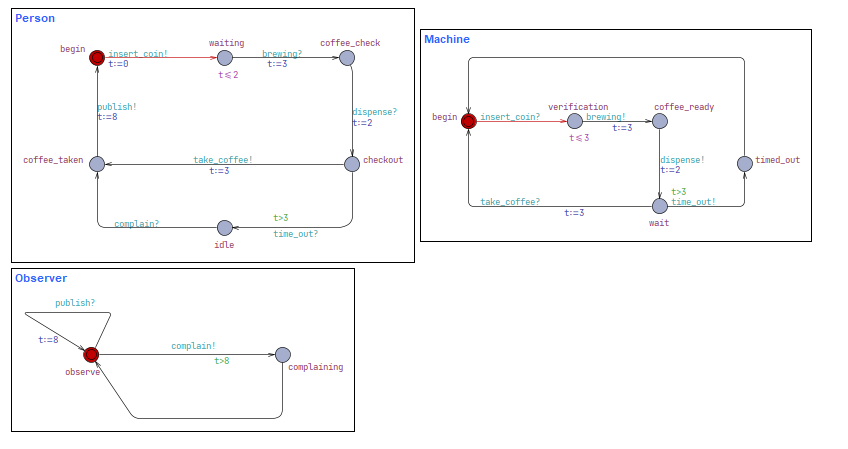
\includegraphics[width=0.9\textwidth]{model-caffee.png} 
    \caption{Model Jaringan Timed Automata untuk Mesin Penjual Kopi di UPPAAL, menunjukkan tiga komponen: Person, Machine, dan Observer.}
    \label{fig:model}
\end{figure}

\section{Hasil dan Pembahasan}
\subsection{Analisis Simulasi}
Simulasi pada UPPAAL digunakan untuk menganalisis perilaku dinamis dari model secara interaktif. Fitur simulator memungkinkan eksekusi langkah-demi-langkah dari sistem, memberikan pemahaman visual tentang bagaimana interaksi antar komponen dan batasan waktu mempengaruhi alur kerja sistem.

Gambar \ref{fig:simulasi} menunjukkan salah satu jejak eksekusi (\textit{trace}) yang mungkin terjadi. Panel "Simulation Trace" di sebelah kiri mencatat urutan transisi yang dieksekusi, seperti \texttt{Person.insert\_coin}, diikuti oleh \texttt{Machine.brewing}, dan diakhiri dengan \texttt{Person.take\_coffee} dan \texttt{Person.publish}. Melalui simulasi, dapat diamati secara visual bahwa pengguna harus menunggu mesin selesai menyeduh sebelum kopi dapat diambil. Skenario lain, seperti mesin mengalami \textit{timeout} karena kopi tidak kunjung diambil, juga dapat dieksplorasi. Simulasi ini berfungsi sebagai langkah validasi awal sebelum verifikasi formal dilakukan.

\begin{figure}[htbp]
    \centering
    % Ganti 'simulasi-caffee.png' dengan path file gambar Anda
    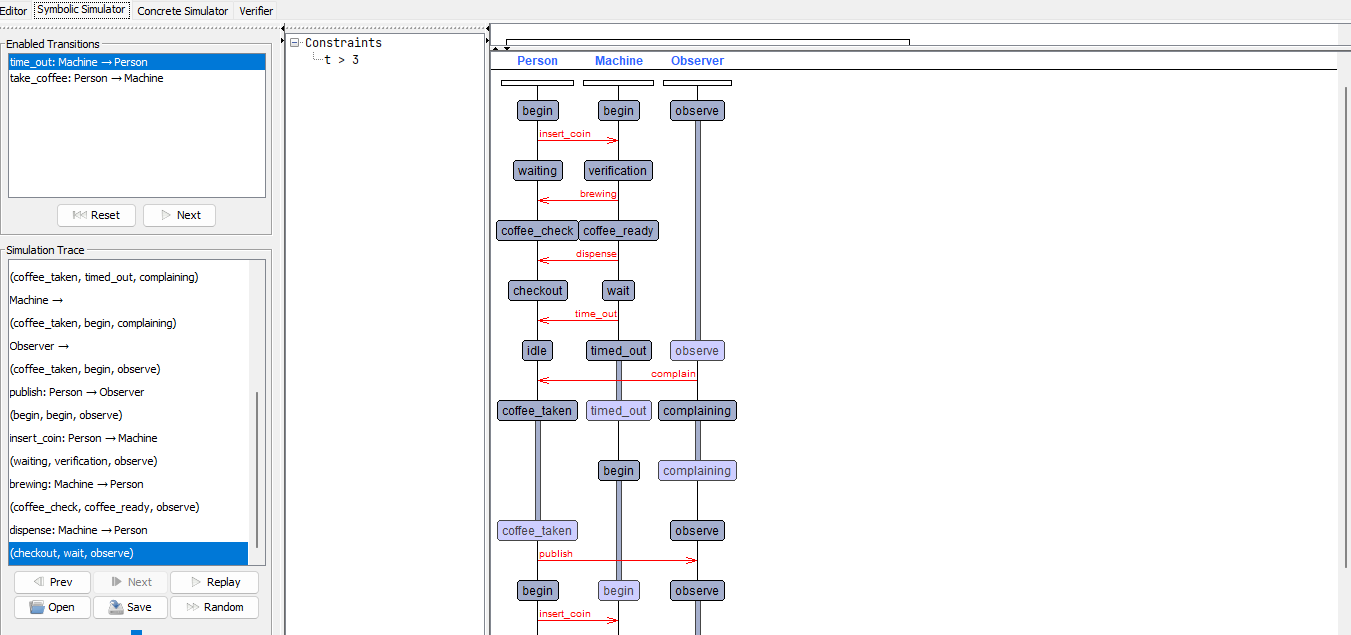
\includegraphics[width=0.8\textwidth]{simulasi-caffee.png}
    \caption{Antarmuka Simulasi di UPPAAL yang menunjukkan jejak eksekusi dari interaksi normal antara pengguna dan mesin.}
    \label{fig:simulasi}
\end{figure}

\subsection{Analisis Verifikasi Formal}
Verifikasi formal dilakukan menggunakan \textit{verifier} di UPPAAL untuk memeriksa kebenaran properti sistem secara menyeluruh terhadap semua kemungkinan jalur eksekusi. Properti-properti ini diekspresikan dalam TCTL. Hasil verifikasi ditampilkan pada Gambar \ref{fig:verifikasi}. Lingkaran hijau menandakan bahwa properti tersebut terbukti benar (\textit{satisfied}).

\begin{figure}[htbp]
    \centering
    % Ganti 'verifikasi-caffee.png' dengan path file gambar Anda
    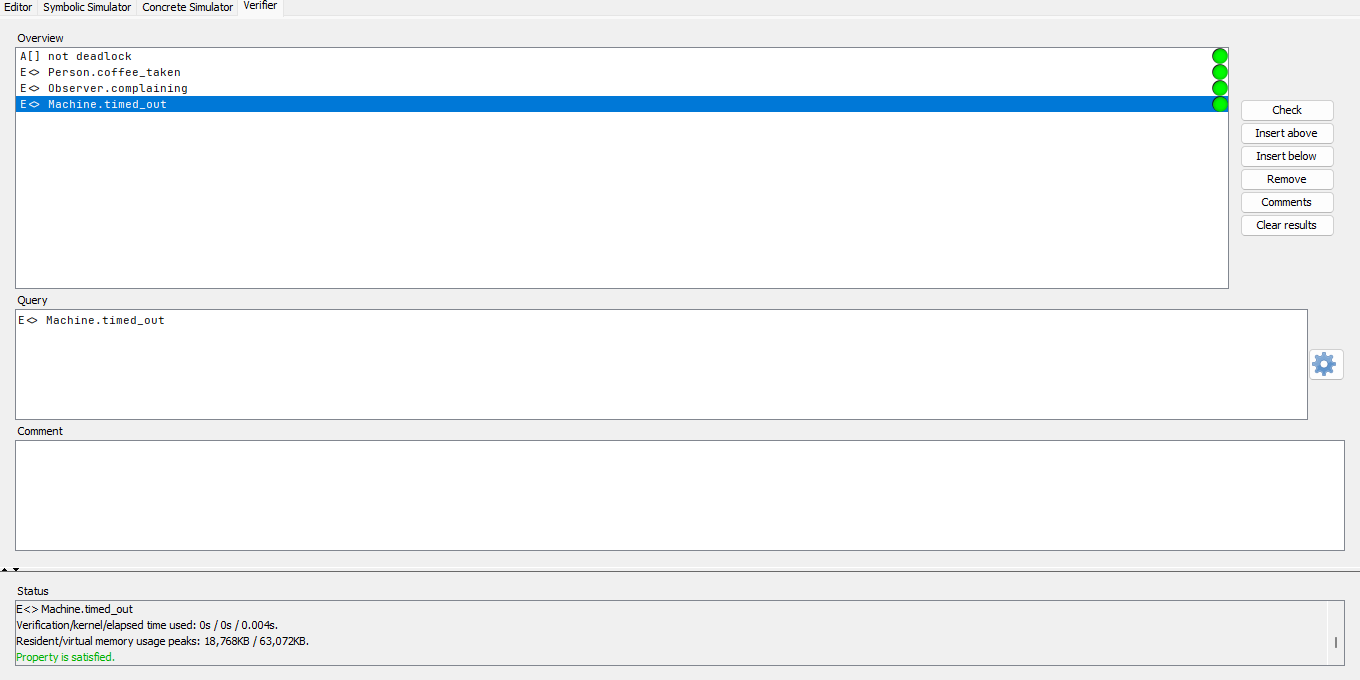
\includegraphics[width=\textwidth]{verifikasi-caffee.png}
    \caption{Hasil verifikasi TCTL pada UPPAAL. Semua properti yang diuji terbukti terpenuhi oleh model.}
    \label{fig:verifikasi}
\end{figure}

Berikut adalah analisis dari setiap properti yang diuji:

\begin{enumerate}
    \item \textbf{A[] not deadlock}: Properti ini adalah properti \textit{safety} fundamental yang memeriksa "untuk semua jalur (\textbf{A}) di semua keadaan (\textbf[]), sistem tidak pernah berada dalam kondisi \textit{deadlock}". Hasil "Property is satisfied" menjamin bahwa model sistem tidak akan pernah mencapai keadaan buntu di mana tidak ada transisi lebih lanjut yang dapat dieksekusi. Ini adalah jaminan vital untuk keandalan sistem.

    \item \textbf{E\textless\textgreater{} Person.coffee\_taken}: Properti \textit{reachability} ini menanyakan "apakah ada (\textbf{E}) setidaknya satu jalur eksekusi di mana pada suatu saat di masa depan (\textbf{\textless\textgreater{}}), keadaan \texttt{Person.coffee\_taken} dapat tercapai?". Hasil yang memuaskan membuktikan bahwa skenario di mana pengguna berhasil mendapatkan kopi adalah mungkin. Ini memvalidasi bahwa fungsi utama dari sistem dapat terpenuhi.

    \item \textbf{E\textless\textgreater{} Observer.complaining}: Properti \textit{reachability} ini memeriksa apakah mekanisme observasi berfungsi seperti yang diharapkan. Pertanyaannya adalah "apakah ada (\textbf{E}) kemungkinan (\textbf{\textless\textgreater{}}) keadaan \texttt{Observer.complaining} tercapai?". Hasil yang memuaskan mengonfirmasi bahwa jika waktu layanan melebihi batas yang ditentukan (8 unit waktu), sistem pengamat akan mendeteksinya. Ini penting untuk menguji logika penanganan kasus-kasus khusus atau kegagalan layanan.

    \item \textbf{E\textless\textgreater{} Machine.time\_out}: Mirip dengan sebelumnya, properti ini memeriksa "apakah ada (\textbf{E}) skenario di mana mesin dapat mencapai (\textbf{\textless\textgreater{}}) keadaan \texttt{time\_out}?". Kepuasan properti ini menunjukkan bahwa logika \textit{timeout} pada mesin telah dimodelkan dengan benar dan dapat terjadi jika kopi tidak diambil dalam batas waktu yang ditentukan.
\end{enumerate}

Hasil verifikasi ini secara kolektif memberikan keyakinan tinggi bahwa model mesin penjual kopi yang dirancang memenuhi spesifikasi fungsional dan temporal yang kunci, termasuk bebas dari deadlock, mampu menyelesaikan transaksi, dan dapat menangani kondisi-kondisi anomali seperti \textit{timeout} dan keterlambatan layanan.

\section{Simpulan}
Penelitian ini telah berhasil mendemonstrasikan penerapan metode formal, khususnya \textit{model checking} dengan Timed Automata, untuk pemodelan dan verifikasi sistem waktu-nyata interaktif. Studi kasus mesin penjual kopi dimodelkan sebagai jaringan Timed Automata menggunakan perangkat bantu UPPAAL, yang mencakup komponen pengguna, mesin, dan pengamat.
Melalui simulasi, perilaku dinamis sistem dapat divalidasi secara visual, sedangkan melalui verifikasi formal, properti-properti penting dapat diuji secara menyeluruh. Hasil verifikasi mengonfirmasi bahwa model yang dibangun memenuhi spesifikasi kunci:
\begin{enumerate}
    \item Sistem dijamin bebas dari \textit{deadlock}.
    \item Skenario keberhasilan transaksi (pengguna mendapatkan kopi) dapat dicapai.
    \item Mekanisme penanganan kondisi khusus seperti \textit{timeout} pada mesin dan deteksi keterlambatan layanan oleh pengamat berfungsi sesuai desain.
\end{enumerate}
Studi ini menunjukkan bahwa pendekatan menggunakan UPPAAL sangat efektif untuk menganalisis dan memvalidasi kebenaran desain sistem sebelum tahap implementasi, sehingga dapat meningkatkan keandalan sistem dan mengurangi potensi biaya perbaikan.

\section*{Ucapan Terima Kasih}
Penulis mengucapkan terima kasih kepada Dr. Dieky Adzkiya, S.Si., M.Si. selaku dosen pengampu mata kuliah Pengantar Verifikasi Sistem yang telah memberikan bimbingan, materi, dan arahan yang sangat berharga dalam penyelesaian studi dan penulisan paper ini.

% Mencetak daftar pustaka
\printbibliography[title={Daftar Pustaka}]

\end{document}